\chapter{Testes e Resultados}
\label{tests:tests}

  \section{Ferramentas de teste}
  \label{tests:tools}

    Para testar a implementação realizada, é necessária uma ferramenta para simular um servidor central. Inicialmente, testou-se a ferramenta \href{http://www.gir.fr/ocppjs/}{GIR OCPPJS}, porém essa apresentou problemas ao lidar com algumas das requisições vindas da \ac{EVSE}.

    Foi criada então uma ferramenta para testes, disponível em \url{https://github.com/brnluiz/ocpp-tools}, que implementa parcialmente as funções de um sistema central. Todas operações apresentadas na tabela \ref{table:ocpp} foram implementadas.

    Após aberta, a ferramenta ouve todas requisições das estações que conectadas e responde as requisições com dados genéricos, o que possibilita o funcionamento da estação protótipo. Caso o desenvolvedor precise executar alguma requisição às estações, é possível utilizar a \ac{CLI} para tal (os comandos disponíveis são dados pelo manual da ferramenta).

  \section{Implementações e testes iniciais}
  \label{tests:initial}

    O desenvolvimento inicial se deu no estudo da base de código anterior, que ainda não implementava nada da \ac{EVSE} funcionalmente, apenas possibilitava o teste de cada dispositivo isoladamente. Após esse período inicial, iniciou-se a implementação do software da estação.

    Alguns testes unitários foram desenvolvidos sob o \textit{framework} de testes \textit{JUnit}, o que permite o programa ser testado antes de ser embarcado. Assim que todos testes passam, o programa é enviado para a \textit{BeagleBone}, a qual está conectada aos dispositivos listados na seção \ref{tests:devices}, porém dispostos em uma bancada de testes (figura \ref{fig:setup-tests}).

    Como as cargas utilizadas durante o teste consumiam pouca energia (fontes \ac{CA}-\ac{CC} de dispositivos de baixo consumo, como notebooks), o medidor de energia teve seu multiplicador de corrente configurado em 100, possibilitando assim simular um consumo alto de forma rápida (sem ter que aguardar várias horas para atingir 1 kWh).

    Todos arquivos, sistema operacional incluso, são colocados em um cartão SD, o que facilita a cópia desses dados para backup (criação de imagens) e permite o intercâmbio do sistema entre a bancada de testes e a estação protótipo.

    \begin{figure}[H]
      \begin{center}
        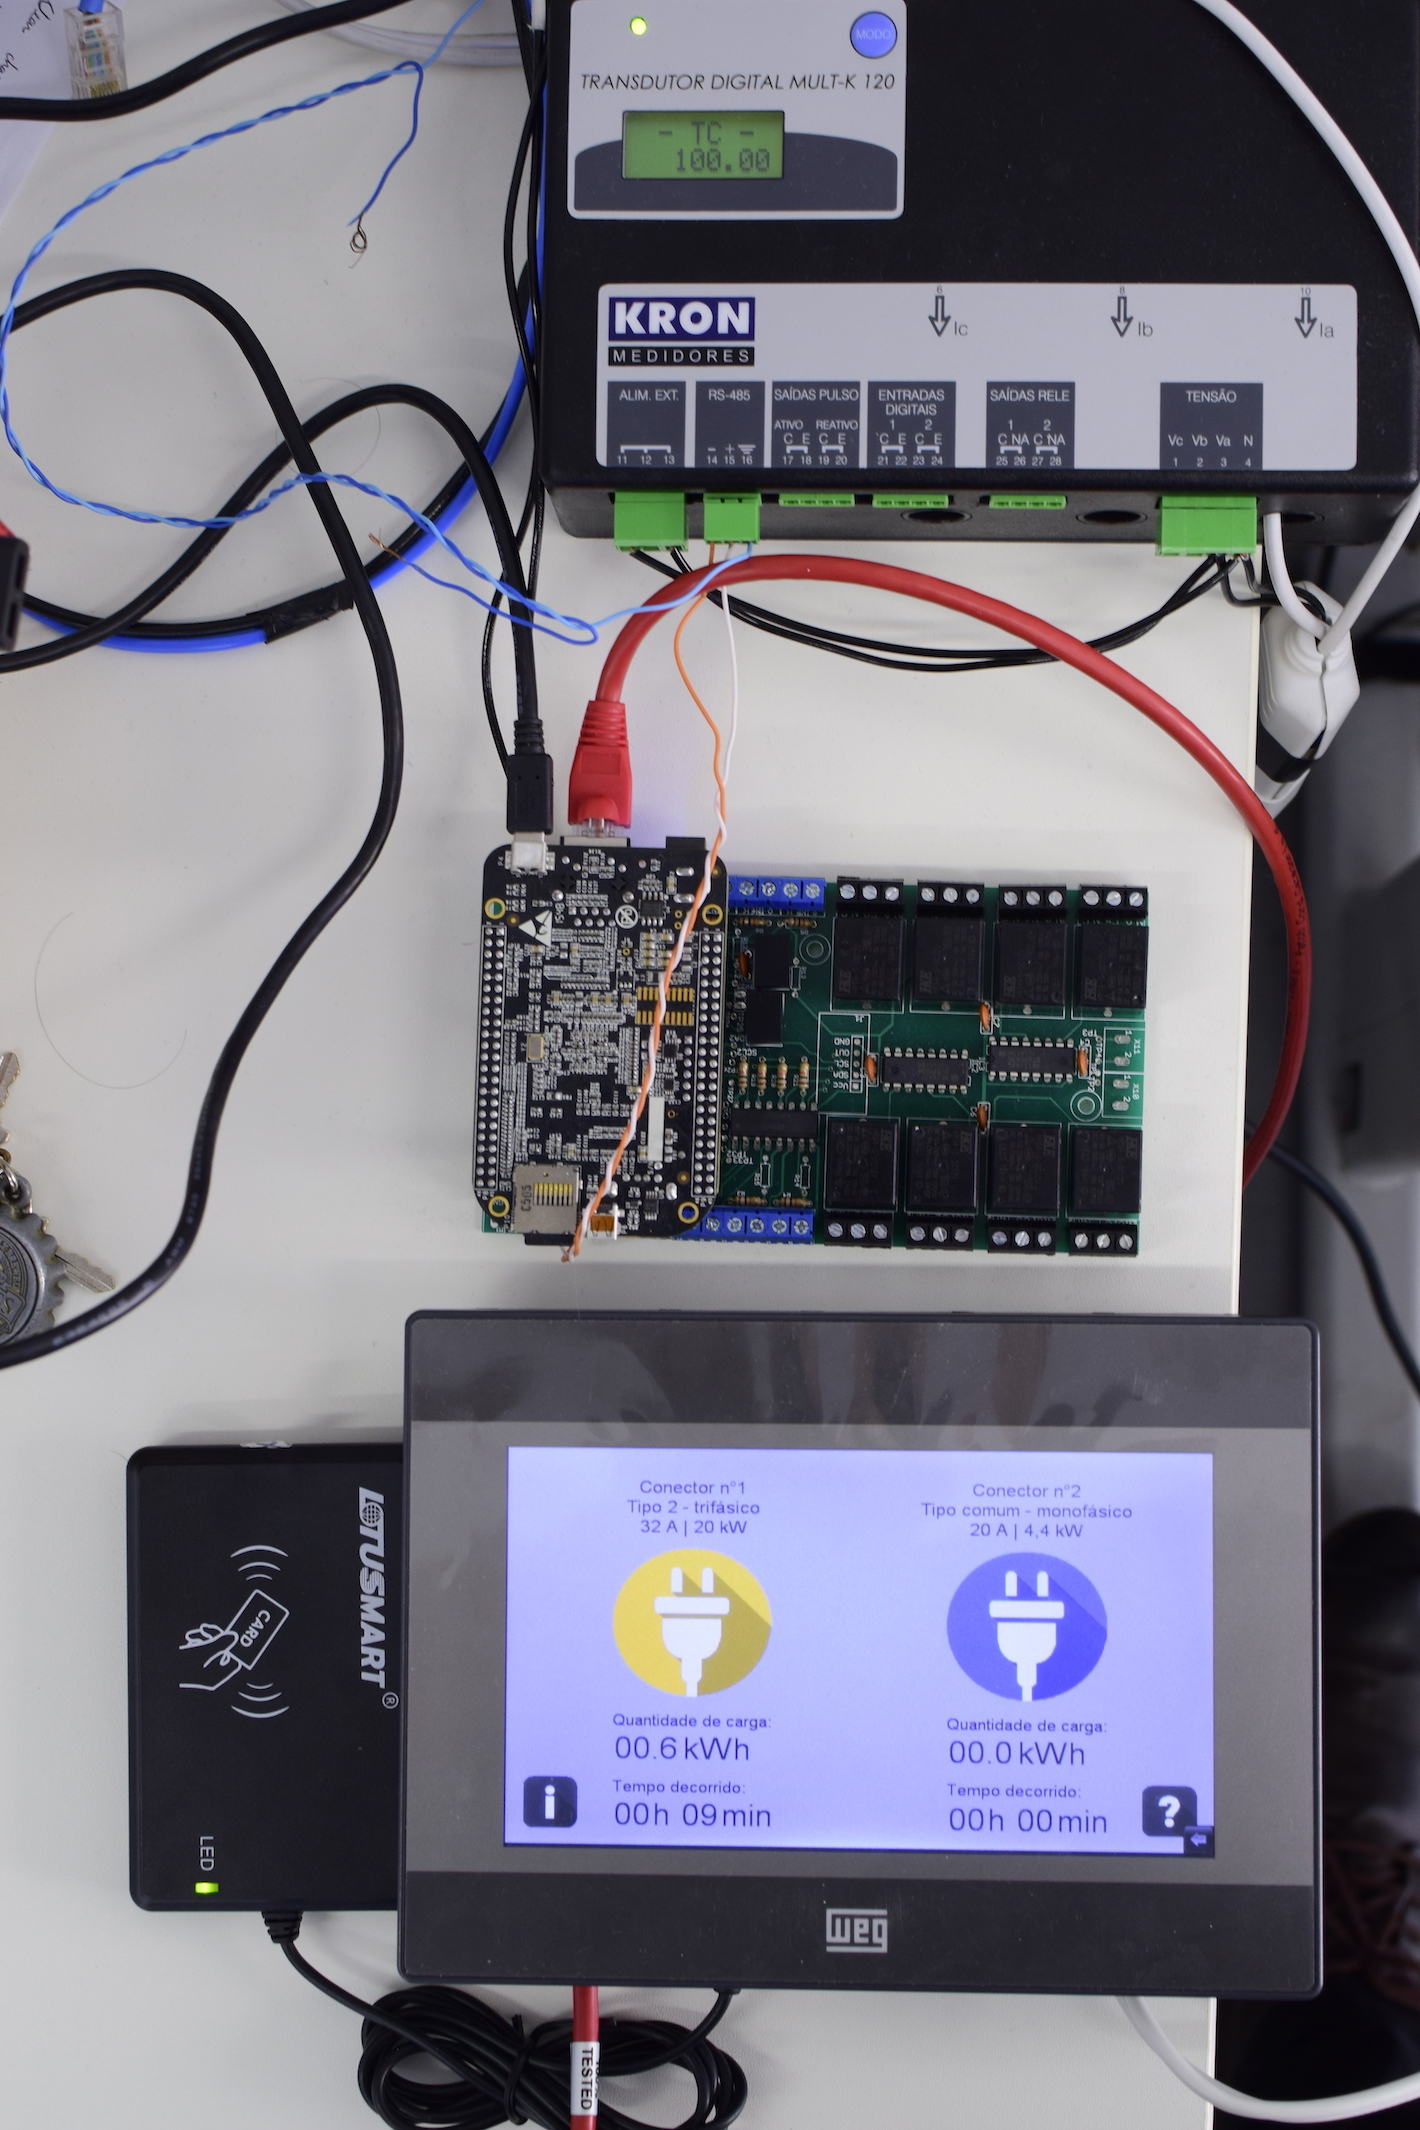
\includegraphics[width=0.6\textwidth,natwidth=2130,natheight=1420,angle=-90]{assets/images/setup-tests.jpg}
        \caption{Disposição dos dispositivos na bancada de testes}
        \label{fig:setup-tests}
      \end{center}
    \end{figure}

  \section{Testes na estação protótipo}
  \label{tests:evse}

    Após diversos testes, o sistema foi levado para a \ac{EVSE} protótipo, situada no estacionamento da Fundação CERTI. A disposição dos dispositivos da estação difere com a da bancada de testes (figura \ref{fig:setup-evse}), porém visto que os dispositivos são os mesmos e o sistema embarcado foi colocado em um cartão SD, só é necessário inserir o cartão na BeagleBone da estação e configurá-la para dar boot pelo cartão, caso já não estiver configurada de fábrica assim.

    \begin{figure}[H]
      \begin{center}
        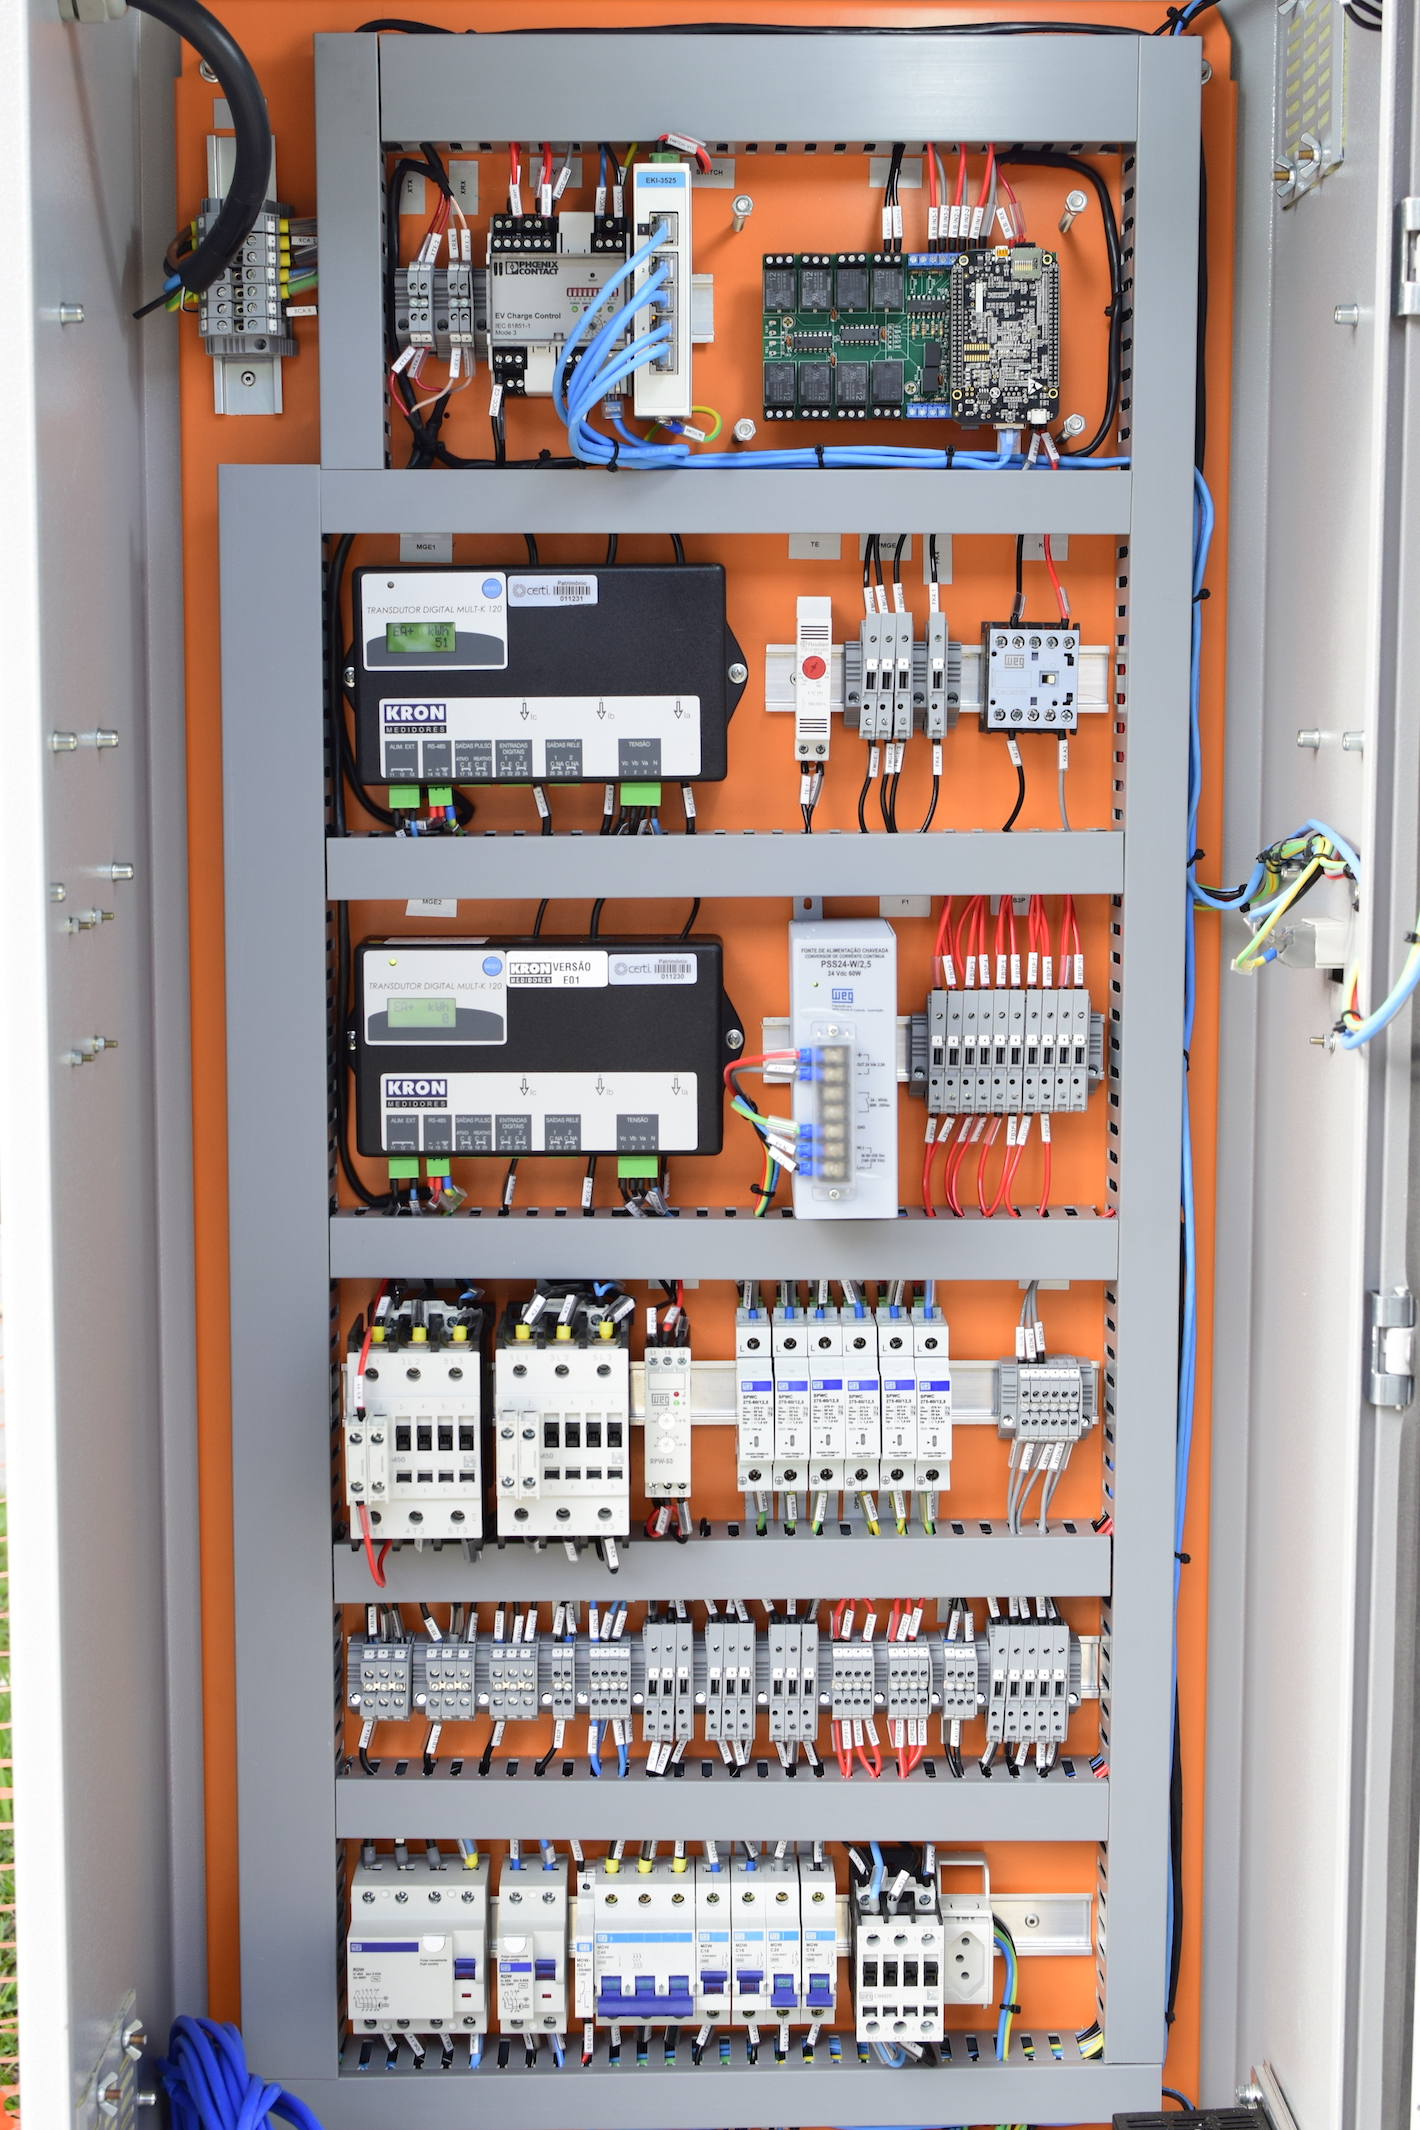
\includegraphics[width=\textwidth,natwidth=1420,natheight=2130]{assets/images/setup-evse.jpg}
        \caption{Disposição dos dispositivos na estação protótipo}
        \label{fig:setup-evse}
      \end{center}
    \end{figure}

    Inicialmente, houveram problemas relativos à configurações de IP estático da BeagleBone da estação e endereçamento dos medidores de energia. O primeiro foi resolvido com a substituição do \textit{connman} e pelo \textit{Network Manager} do Linux embarcado. Já o segundo era um problema na configuração do endereço MODBUS e das configurações seriais, onde foi necessário readequar os parâmetros do sistema embarcado para os da \textit{\ac{EVSE}}. 

    Após resolvidos, a \textit{\ac{EVSE}} funcionou da mesma maneira que funcionava na bancada de testes, o que finaliza as entregas do projeto.
